%%%%%%%%%%%%%%%%%%% EJERCICIO 9.d  %%%%%%
\textbf{Parte d.} Una tasa nominal anual semestre anticipado. \\
%\newpage %USAR SOLO SI EL SOLUCIÓN QUEDA SOLO Y ES NECESARIO BAJARLO A LA SIGUIENTE PAGINA
\textbf{Solución d.}\\
%La tabla ira centrada
\begin{center}
   \renewcommand{\arraystretch}{1.5}% Margenes de las celdas
   %Creación de la cuadricula de 3 columnas
   \begin{longtable}[H]{|c|c|c|}
      %Creamos una linea horizontal
      \hline
      %Definimos el color de la primera fila
      \rowcolor[HTML]{FFB183}
      %%%%% INICIO ASIGNACIÓN PERíODO FOCAL %%%%%%%
      %%%%%%%%%% INICIO TITULO
      %Lo que se hace aquí es mezclar las 3 columnas en una sola
      \multicolumn{3}{|c|}{\cellcolor[HTML]{FFB183}\textbf{1. Asignación período focal}}                                                                                                                   \\ \hline
      \multicolumn{3}{|c|}{$pf= \textit{No aplica}$}                                                                                                                                              
      \\ \hline
      %%%%%%%%%% FIN TITULO
      %%%%% INICIO DECLARACIÓN DE VARIABLES %%%%%%%
      %%%%%%%%%% INICIO TITULO
      %Lo que se hace aquí es mezclar las 3 columnas en una sola
      \multicolumn{3}{|c|}{\cellcolor[HTML]{FFB183}\textbf{2. Declaración de variables}}                                                                                                                       \\ \hline
      %%%%%%%%%% FIN TITULO
      %%%%%%%%%% INICIO DE MATEMÁTICAS
      %Cada & hace referencia al paso de la siguiente columna
      $j_{1} = 24\% \textit{ namv}$ & $m_{1} = 12  \textit{ pmv}  $  & $i_{2} = ?\% \textit{ psv} $ \\ 
      $i_{1} = 2\% \textit{ pmv}$ & $m_{2} = 2 \textit{ psa} $     &  $i_{a2} = ?\% \textit{ psa} $  \\
       &         & $j_{a2} = ?\% \textit{ nasa} $                \\ \hline
      %%%%%%%%%% FIN DE MATEMÁTICAS
      %%%%% FIN DECLARACIÓN DE VARIABLES

      %%%%% INICIO FLUJO DE CAJA
      \rowcolor[HTML]{FFB183}
      \multicolumn{3}{|c|}{\cellcolor[HTML]{FFB183}\textbf{3. Diagrama de equivalencia de tasas}}                                                                                                              \\ \hline
      %Mezclamos 3 columnas y pondremos el dibujo
      %%%%%%%%%%%%% INSERCIÓN DE LA IMAGEN
      %Deberán descargar las imágenes respectivas del drive y pegarlas en la carpeta
      %n_capitulo/img/ejemplos/1/capitulo1ejemplo1.pdf  (el /1/ es el numero del ejemplo)

      \multicolumn{3}{|c|}{ 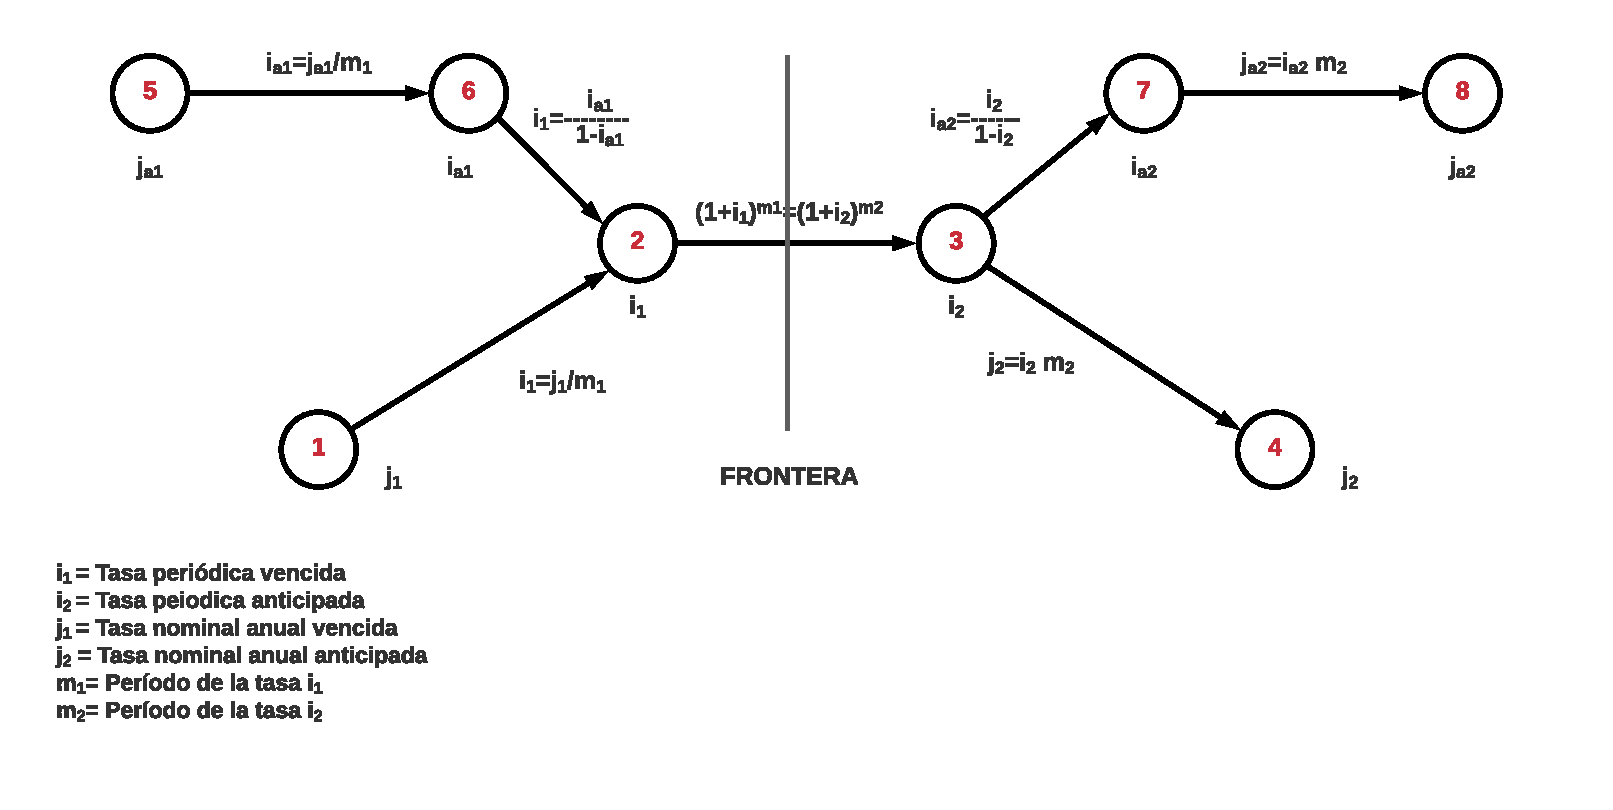
\includegraphics[trim=-5 -5 -5 -5 , scale=0.4]{2_Capitulo/img/ejemplos/6/Capitulo2Ejemplo6.pdf} }  \\ \hline
      
      %%%%%%%%%%%%% FIN INSERCIÓN DE IMAGEN
      %%%%%FIN FLUJO DE CAJA

      %%%%% INICIO DECLARACIÓN FORMULAS
      %%%%%%%%%%% INICIO TITULO
      \rowcolor[HTML]{FFB183}
      \multicolumn{3}{|c|}{\cellcolor[HTML]{FFB183}\textbf{4. Declaración de fórmulas}}                                                                                                                        \\ \hline
      %%%%%%%%%%% FIN TITULO
      %%%%%%%%%%% INICIO MATEMÁTICAS

      \multicolumn{2}{|c|}{ $ (1+i_{1})^{m_{1}}=(1+i_{2})^{m_{2}} \textit{ Equivalencia de tasas}$}      & $j_{a2}=i_{a2}\cdot m_{2} \textit{ Tasa nominal anual anticipada}$                                  \\ \multicolumn{2}{|c|}{$i_{a2} = \frac{i_{2}}{1+i_{2}} \textit{ Tasa periódica anticipada}$}           & \\ \hline
      %%%%%%%%%% FIN MATEMÁTICAS
      %%%%%% INICIO DESARROLLO MATEMÁTICO
      \rowcolor[HTML]{FFB183}
      %%%%%%%%%%INICIO TITULO
      \multicolumn{3}{|c|}{\cellcolor[HTML]{FFB183}\textbf{5. Desarrollo matemático}}                                                                                                                          \\ \hline
      %%%%%%%%%% FIN TITULO
      %%%%%%%%%% INICIO MATEMÁTICAS
      \multicolumn{2}{|c|}{$(1 + 0,02\%)^{12}= (1 + i_{2})^{2} $}                                    & {$j_{a2}=(11,20286178\% \textit{ pbv})(2\textit{ psv})$}                                                                  \\
      \multicolumn{2}{|c|}{$(1,02)^{6}-1=i_{2}$ }                                         & {$j_{a2} = 22,406\% \textit{ nasa}$}                                                                                                     \\
      \multicolumn{2}{|c|}{$i_{2}= 0,12616 \equiv 12,616\% \textit{ psv}$}                                      &                                                                                                     \\
      \multicolumn{2}{|c|}{$i_{a2}=\frac{0,126162419}{1+0,126162419}= 0,11203 \textit{ psa} \equiv 11,203\% \textit{ psa}$} &                                                                                                                                                                      \\ \hline

      %%%%%%%%%% FIN MATEMÁTICAS
      %%%%%% FIN DESARROLLO MATEMÁTICO
      %%%%%% INICIO RESPUESTA
      \rowcolor[HTML]{FFB183}
      %%%%%%%%%%INICIO TITULO
      \multicolumn{3}{|c|}{\cellcolor[HTML]{FFB183}\textbf{6. Respuesta}}                                                                                                                                      \\ \hline
      %%%%%%%%%% FIN TITULO
      %%%%%%%%%% INICIO RESPUESTA MATEMÁTICA
      \multicolumn{3}{|c|}{
         \begin{minipage}[t][0.03\textheight][c]{0.8\columnwidth}
            \centering
            ${j_{a2} = 22,406\% nasa}$
         \end{minipage}
      }   

                                                \\ \hline
      
      %%%%%%%%%% FIN MATEMÁTICAS
      %%%%%% FIN RESPUESTA
   \end{longtable}
   %Se crean dos lineas en blanco para que no quede el siguiente texto tan pegado
   %\newline \newline %USARLO SI CREES QUE ES NECESARIO
\end{center}
%%%%%%%%%%%%%%%%%%% FIN EJERCICIO 9.d  %%%%%%%%%%%%%%%%%%%%%%%%%%%%%%
%%%%%%%%%%%%%%%%%%%%%%%%%%FIN EJERCICIO 9 %%%%%%%%%%%%%%%%%%%%%%%%%%%